\documentclass[14pt,fleqn]{extarticle}
\RequirePackage{prepwell-eng}

\previewoff 

\begin{document} 
\begin{snippet}
    
    \incorrect
    
    Below is the graph of some function $f(x)$. $AB \parallel x-$ axis\newline 
    
    And $f(x)$ is a strictly increasing function 
    
    \begin{center}
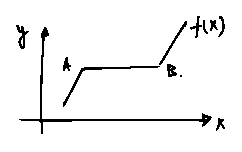
\includegraphics[scale=1.5]{figure.eps}
\end{center}
    \reason
    
    $AB \parallel x-$axis $\implies \dydx = 0$ between $A$ and $B$. Hence, while $f(x)$ is an increasing function, it is \underline{not strictly increasing}\newline 
    
    A function is strictly increasing (in some domain) if $\dydx > 0$ but not $\geq 0$ 
    
\end{snippet} 
\end{document} 